\section{Hastighetsregulator}\label{sec:hastighetsreg}

\subsection{Teori}

Regulatorer brukes for å styre tilstander i en prosess. En regulator regulator får inn et avvik mellom referansen og den målte tilstanden. Regulatorer bruker avviket til å beregne et pådrag til prosessen. P-regulator er en type regulator som lager et pådrag, $u$,  som er proposjonalt med avviket, $e = \omega_d - \omega_m$. $K_p$ er proposjonalitetsleddet i regulatoren, sammenhengen er vist i \autoref{eq:P_regulator}.

\begin{equation}
    \label{eq:P_regulator}
    u(t) = K_p e(t)
\end{equation}

En slik regulator er effektiv så lenge det ikke er en kraft som forhindrer systemet å oppnå en spesifikk tilstand. I et slikt tilfelle vil ikke regulatoren regulere tilstanden til referanseverdien og det til oppstå et stasjonærtavvik. Et integratorledd vil forhindre stasjonærtavvik ved å gi et pådrag som er likt den kraften som forhindrer at systemet når referanse tilstanden. \autoref{eq:PI_regulator} beskriver en PI-regulator,

\begin{equation}
    \label{eq:PI_regulator}
    u(t) = K_p e(t) + \frac{K_p}{T_i} \int_{0}^{t} e(\tau) d\tau
\end{equation}

der $u$ er pådraget, $K_p$ er proposjonalitetskontanten, $e$ er avviket mellom referansen og tilstanden og $T_i$ er integratorkonstanten som representerer tidskonstanten til regulatoren.

\subsection{Metode}

\begin{figure}[b]
    \centering
    \begin{circuitikz} [scale=0.5, transform shape]
    \ctikzset{resistor = european}

    % --- OP1 ---
    \node[op amp](OP1) {$OP1$};
    
    \draw (OP1.-)
    to[R, l_=$R_1$] ++(-2, 0)
    to[short, o-, l=$\omega_m$] ++(0, 0);

    \draw (OP1.+)
    to[R=$R_1$] ++(-2, 0)
    to[short, o-, l=$\omega_d$] ++(0, 0);

    \draw (OP1.+)
    to[R=$R_2$, *-] ++(0, -2)
    node[ground] {};

    \draw (OP1.-)
    to[short, *-] ++(0, 1)
    coordinate(t1)
    to[R=$R_2$] (t1 -| OP1.out)
    -- (OP1.out);

    % --- OP2 ---

    \draw (OP1.out)
    to[short, *-, l=$e$] ++(0.5, 0)
    to[R=$R_3$] ++(2, 0)
    node[op amp, anchor=-](OP2) {$OP2$};

    \draw (OP2.-)
    to[short, *-] ++(0, 1)
    coordinate(t2)
    to[R=$R_4$] (t2 -| OP2.out)
    -- (OP2.out);

    \draw (OP2.+)
    node[ground] {};

    \draw (OP2.out)
    to[short, *-] ++(0, 0)
    to[R=$R_7$] ++(0, -2)
    coordinate(t7);

    % --- OP3 ---

    \draw (OP1.out)
    -- ++(0, -2)
    to[potentiometer, n=R5, l=$R_5$] ++(0, -2)
    coordinate(t3);

    \draw (R5.wiper)
    -- (R5.wiper |- t3)
    -- (t3);

    \draw (t3)
    to[short, *-] ++(0, -1)
    to[R=$R_6$] ++(2, 0)
    node[op amp, anchor=-](OP3) {$OP3$};

    \draw (OP3.+)
    node[ground] {};
    
    \draw (OP3.-)
    to[short, *-] ++(0, 1)
    coordinate(t4)
    to[C=$C_1$] (t4 -| OP3.out)
    coordinate(t5)
    -- (OP3.out);

    \draw (t4)
    to[short, *-] ++(0, 1.3)
    coordinate(t6)
    to[open jumper, l=$JP1$] (t6 -| t5)
    to[short, -*] (t5);

    \draw (OP3.out)
    to[short, *-] (OP3.out -| OP2.out)
    to[R, l_=$R_7$] ++(0, 2)
    coordinate (t8)
    to[short, *-*] (t7);

    % --- OP4 ---

    \draw (t8)
    -- ++(1.5, 0)
    node[op amp, anchor=-](OP4) {$OP4$};

    \draw (OP4.+)
    node[ground] {};

    \draw (t7)
    to[R=$R_8$] ++(2, 0)
    coordinate(t9)
    to[potentiometer, n=R9, l=$R_9$] (t9 -| OP4.out)
    coordinate(t10)
    -- (OP4.out);

    \draw (R9.wiper)
    -- (R9.wiper -| t10)
    to[short, -*] (t10);

    \draw (OP4.out)
    to[short, *-o, l=$V_m$] ++(1, 0);
    
\end{circuitikz}
    \caption{PI-regulator krets for hastighetsregulatoren. Hentet fra \cite{AnalogMotorlabbOppgaver}}
    \label{fig:krets_hastighets_regulator}
\end{figure}

Hastighetsregulatoren ble implementer som en analog PI-regulator som vist i \autoref{fig:krets_hastighets_regulator}. $OP1$ er en differensialforsterker som finner avviket, $e$, transferfunksjonen er gitt ved \autoref{eq:differensialforsterker}.
$OP2$ er en inverterende forsterker som inverterer avviket, uten forsterkning eller demping.
$OP3$ er en integrerende forsterker som integrerer $e$ og forsterker den med $\frac{1}{T_i}$. $JP1$ brukes for å nullstille integratoren og skru av I-leddet i integratoren. Transferfunksjonen til $OP3$ er $-\frac{1}{(R_5 + R_6) C_1} \int e dt$.
$OP4$ summerer spenningen fra $OP2$ og $OP3$ og forsterker resultatet med $K_p$. Transferfunksjonen for $OP4$ er $-\frac{R_8 + R_9}{R_7}(v_2 + v_3)$, der $v_2$ er spenningen ut av $OP2$ og $v_3$ er spenningen ut av $OP3$. Ut fra dette finner vi uttrykk for $K_p$ og $T_i$ som vist i \autoref{eq:K_p_og_T_i}.

\begin{equation}
    \label{eq:K_p_og_T_i}
    K_p = \frac{R_2}{R_1} \frac{R_8 + R_9}{R_7},
    T_i = (R_5 + R_6) C_1
\end{equation}

Størrelsen på motstandene og kondensatoren er vist i \autoref{tab:Komponenter_i_hastighetsregulatoren}

\begin{table}
    \centering
    \caption{Motstander og kondensatorer i hastighetsregulatoren. Verdiene er hentet fra \cite{AnalogMotorlabbOppgaver}}
    \begin{tabular}{lll}
        \toprule
        Størrelse & Verdi & Type \\
		\midrule
        $R_1$, $R_2$ & $100\,k\Omega$ & Resistor\\
        $R_3$, $R_4$, $R_7$, $R_8$ & $10\,k\Omega$ & Resistor \\
        $R_5$, $R_9$ & $1\,M\Omega$ & Potmeter \\
        $R_6$ & $1\,k\Omega$ & Resistor \\
        $C_1$ & $1\,\mu F$ & Kondensator \\
        \bottomrule
    \end{tabular}
    \label{tab:Komponenter_i_hastighetsregulatoren}
\end{table}

\subsection{Resultater}

\begin{figure}
    \centering
    % This file was created with tikzplotlib v0.10.1.
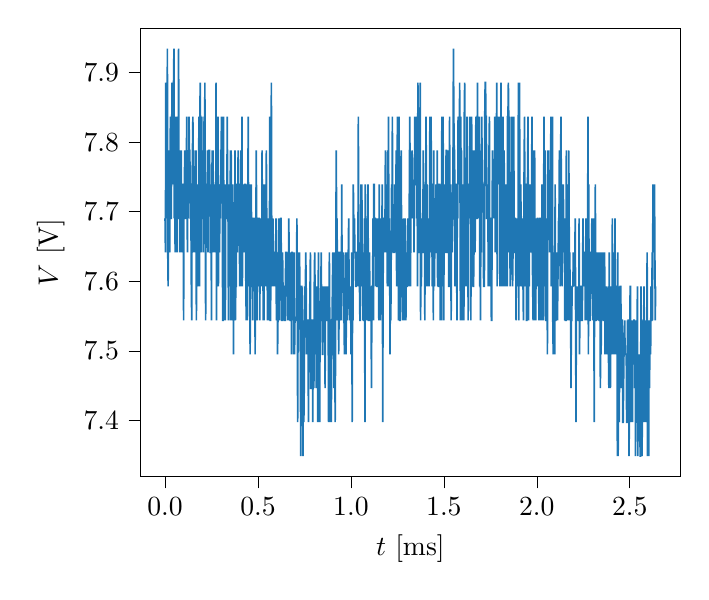
\begin{tikzpicture}

\definecolor{darkgray176}{RGB}{176,176,176}
\definecolor{steelblue31119180}{RGB}{31,119,180}

\begin{axis}[
tick align=outside,
tick pos=left,
x grid style={darkgray176},
xlabel={\(\displaystyle t\) [ms]},
xmin=-0.131976, xmax=2.771496,
xtick style={color=black},
xtick={-0.5,0,0.5,1,1.5,2,2.5,3},
xticklabels={
  \(\displaystyle {\ensuremath{-}0.5}\),
  \(\displaystyle {0.0}\),
  \(\displaystyle {0.5}\),
  \(\displaystyle {1.0}\),
  \(\displaystyle {1.5}\),
  \(\displaystyle {2.0}\),
  \(\displaystyle {2.5}\),
  \(\displaystyle {3.0}\)
},
y grid style={darkgray176},
ylabel={\(\displaystyle V\) [V]},
ymin=7.319333, ymax=7.963867,
ytick style={color=black},
ytick={7.3,7.4,7.5,7.6,7.7,7.8,7.9,8},
yticklabels={
  \(\displaystyle {7.3}\),
  \(\displaystyle {7.4}\),
  \(\displaystyle {7.5}\),
  \(\displaystyle {7.6}\),
  \(\displaystyle {7.7}\),
  \(\displaystyle {7.8}\),
  \(\displaystyle {7.9}\),
  \(\displaystyle {8.0}\)
}
]
\addplot [semithick, steelblue31119180]
table {%
0 7.69043
0.00208000000000001 7.6416
0.00416000000000001 7.88574
0.00624000000000002 7.83691
0.00832000000000003 7.83691
0.0103999999999998 7.69043
0.0124799999999998 7.93457
0.0145599999999998 7.6416
0.0166399999999998 7.59277
0.0187199999999998 7.73926
0.0207999999999999 7.6416
0.0228799999999999 7.78809
0.0249599999999999 7.6416
0.0270399999999999 7.78809
0.0291199999999999 7.83691
0.0311999999999999 7.69043
0.0332799999999999 7.69043
0.0353599999999999 7.78809
0.0374399999999999 7.88574
0.0395199999999999 7.78809
0.0415999999999999 7.83691
0.0436799999999999 7.73926
0.0457599999999999 7.88574
0.04784 7.93457
0.04992 7.69043
0.052 7.83691
0.05408 7.6416
0.05616 7.78809
0.05824 7.73926
0.06032 7.78809
0.0624 7.83691
0.06448 7.6416
0.06656 7.83691
0.06864 7.69043
0.07072 7.69043
0.0727999999999998 7.93457
0.0748799999999998 7.73926
0.0769599999999998 7.78809
0.0790399999999998 7.6416
0.0811199999999998 7.69043
0.0831999999999999 7.69043
0.0852799999999999 7.6416
0.0873599999999999 7.78809
0.0894399999999999 7.6416
0.0915199999999999 7.69043
0.0935999999999999 7.73926
0.0956799999999999 7.73926
0.0977599999999999 7.73926
0.0998399999999999 7.54395
0.10192 7.73926
0.104 7.73926
0.10608 7.78809
0.10816 7.73926
0.11024 7.69043
0.11232 7.69043
0.1144 7.73926
0.11648 7.83691
0.11856 7.69043
0.12064 7.6416
0.12272 7.73926
0.1248 7.69043
0.12688 7.73926
0.12896 7.83691
0.13104 7.78809
0.13312 7.78809
0.1352 7.73926
0.13728 7.69043
0.13936 7.69043
0.14144 7.59277
0.14352 7.54395
0.1456 7.73926
0.14768 7.78809
0.14976 7.83691
0.15184 7.73926
0.15392 7.6416
0.156 7.69043
0.15808 7.6416
0.16016 7.69043
0.16224 7.78809
0.16432 7.73926
0.1664 7.78809
0.16848 7.54395
0.17056 7.6416
0.17264 7.69043
0.17472 7.73926
0.1768 7.6416
0.17888 7.59277
0.18096 7.78809
0.18304 7.83691
0.18512 7.59277
0.1872 7.83691
0.18928 7.88574
0.19136 7.78809
0.19344 7.6416
0.19552 7.78809
0.1976 7.83691
0.19968 7.69043
0.20176 7.69043
0.20384 7.78809
0.20592 7.6416
0.208 7.69043
0.21008 7.83691
0.21216 7.69043
0.21424 7.88574
0.21632 7.69043
0.2184 7.54395
0.22048 7.69043
0.22256 7.69043
0.22464 7.73926
0.22672 7.73926
0.2288 7.78809
0.23088 7.6416
0.23296 7.73926
0.23504 7.78809
0.23712 7.78809
0.2392 7.78809
0.24128 7.73926
0.24336 7.6416
0.24544 7.6416
0.24752 7.73926
0.2496 7.54395
0.25168 7.73926
0.25376 7.78809
0.25584 7.6416
0.25792 7.78809
0.26 7.69043
0.26208 7.73926
0.26416 7.6416
0.26624 7.69043
0.26832 7.6416
0.2704 7.69043
0.27248 7.69043
0.27456 7.88574
0.27664 7.54395
0.27872 7.73926
0.2808 7.78809
0.28288 7.73926
0.28496 7.83691
0.28704 7.59277
0.28912 7.69043
0.2912 7.69043
0.29328 7.6416
0.29536 7.73926
0.29744 7.69043
0.29952 7.78809
0.3016 7.78809
0.30368 7.83691
0.30576 7.73926
0.30784 7.78809
0.30992 7.54395
0.312 7.54395
0.31408 7.83691
0.31616 7.69043
0.31824 7.73926
0.32032 7.54395
0.3224 7.73926
0.32448 7.54395
0.32656 7.73926
0.32864 7.69043
0.33072 7.69043
0.3328 7.73926
0.33488 7.83691
0.33696 7.69043
0.33904 7.69043
0.34112 7.54395
0.3432 7.73926
0.34528 7.69043
0.34736 7.69043
0.34944 7.59277
0.35152 7.78809
0.3536 7.54395
0.35568 7.78809
0.35776 7.54395
0.35984 7.73926
0.36192 7.59277
0.364 7.73926
0.36608 7.6416
0.36816 7.49512
0.37024 7.6416
0.37232 7.69043
0.3744 7.6416
0.37648 7.78809
0.37856 7.54395
0.38064 7.59277
0.38272 7.59277
0.3848 7.73926
0.38688 7.73926
0.38896 7.6416
0.39104 7.69043
0.39312 7.78809
0.3952 7.69043
0.39728 7.73926
0.39936 7.73926
0.40144 7.59277
0.40352 7.73926
0.4056 7.59277
0.40768 7.78809
0.40976 7.6416
0.41184 7.69043
0.41392 7.83691
0.416 7.59277
0.41808 7.69043
0.42016 7.6416
0.42224 7.69043
0.42432 7.73926
0.4264 7.6416
0.42848 7.73926
0.43056 7.73926
0.43264 7.73926
0.43472 7.59277
0.4368 7.54395
0.43888 7.73926
0.44096 7.69043
0.44304 7.54395
0.44512 7.6416
0.4472 7.83691
0.44928 7.69043
0.45136 7.59277
0.45344 7.69043
0.45552 7.73926
0.4576 7.49512
0.45968 7.59277
0.46176 7.59277
0.46384 7.73926
0.46592 7.6416
0.468 7.6416
0.47008 7.6416
0.47216 7.54395
0.47424 7.69043
0.47632 7.69043
0.4784 7.69043
0.48048 7.59277
0.48256 7.69043
0.48464 7.49512
0.48672 7.69043
0.4888 7.69043
0.49088 7.78809
0.49296 7.6416
0.49504 7.54395
0.49712 7.69043
0.4992 7.69043
0.50128 7.69043
0.50336 7.59277
0.50544 7.69043
0.50752 7.69043
0.5096 7.54395
0.51168 7.6416
0.51376 7.69043
0.51584 7.59277
0.51792 7.69043
0.52 7.6416
0.52208 7.78809
0.52416 7.59277
0.52624 7.6416
0.52832 7.54395
0.5304 7.73926
0.53248 7.54395
0.53456 7.69043
0.53664 7.6416
0.53872 7.59277
0.5408 7.73926
0.54288 7.6416
0.54496 7.78809
0.54704 7.69043
0.54912 7.6416
0.5512 7.54395
0.55328 7.69043
0.55536 7.59277
0.55744 7.69043
0.55952 7.54395
0.5616 7.6416
0.56368 7.83691
0.56576 7.54395
0.56784 7.54395
0.56992 7.69043
0.572 7.88574
0.57408 7.6416
0.57616 7.6416
0.57824 7.59277
0.58032 7.69043
0.5824 7.6416
0.58448 7.6416
0.58656 7.6416
0.58864 7.59277
0.59072 7.6416
0.5928 7.6416
0.59488 7.6416
0.59696 7.69043
0.59904 7.54395
0.60112 7.59277
0.6032 7.6416
0.60528 7.49512
0.60736 7.54395
0.60944 7.6416
0.61152 7.69043
0.6136 7.6416
0.61568 7.54395
0.61776 7.69043
0.61984 7.6416
0.62192 7.69043
0.624 7.69043
0.62608 7.59277
0.62816 7.54395
0.63024 7.54395
0.63232 7.6416
0.6344 7.59277
0.63648 7.54395
0.63856 7.59277
0.64064 7.59277
0.64272 7.54395
0.6448 7.54395
0.64688 7.54395
0.64896 7.6416
0.65104 7.6416
0.65312 7.6416
0.6552 7.59277
0.65728 7.6416
0.65936 7.54395
0.66144 7.59277
0.66352 7.54395
0.6656 7.69043
0.66768 7.6416
0.66976 7.59277
0.67184 7.6416
0.67392 7.54395
0.676 7.54395
0.67808 7.6416
0.68016 7.49512
0.68224 7.6416
0.68432 7.6416
0.6864 7.54395
0.68848 7.59277
0.69056 7.59277
0.69264 7.49512
0.69472 7.6416
0.6968 7.49512
0.69888 7.54395
0.70096 7.54395
0.70304 7.54395
0.70512 7.54395
0.7072 7.54395
0.70928 7.69043
0.71136 7.59277
0.71344 7.39746
0.71552 7.54395
0.7176 7.59277
0.71968 7.6416
0.72176 7.59277
0.72384 7.6416
0.72592 7.54395
0.728 7.49512
0.73008 7.34863
0.73216 7.44629
0.73424 7.59277
0.73632 7.59277
0.7384 7.54395
0.74048 7.49512
0.74256 7.34863
0.74464 7.54395
0.74672 7.39746
0.7488 7.44629
0.75088 7.59277
0.75296 7.54395
0.75504 7.59277
0.75712 7.6416
0.7592 7.59277
0.76128 7.49512
0.76336 7.54395
0.76544 7.54395
0.76752 7.54395
0.7696 7.49512
0.77168 7.39746
0.77376 7.54395
0.77584 7.49512
0.77792 7.54395
0.78 7.59277
0.78208 7.6416
0.78416 7.44629
0.78624 7.44629
0.78832 7.54395
0.7904 7.54395
0.79248 7.54395
0.79456 7.39746
0.79664 7.49512
0.79872 7.49512
0.8008 7.44629
0.80288 7.59277
0.80496 7.6416
0.80704 7.59277
0.80912 7.49512
0.8112 7.59277
0.81328 7.44629
0.81536 7.59277
0.81744 7.44629
0.81952 7.54395
0.8216 7.39746
0.82368 7.59277
0.82576 7.6416
0.82784 7.44629
0.82992 7.49512
0.832 7.39746
0.83408 7.54395
0.83616 7.54395
0.83824 7.59277
0.84032 7.6416
0.8424 7.54395
0.84448 7.59277
0.84656 7.49512
0.84864 7.49512
0.85072 7.54395
0.8528 7.54395
0.85488 7.59277
0.85696 7.54395
0.85904 7.54395
0.86112 7.44629
0.8632 7.59277
0.86528 7.54395
0.86736 7.54395
0.86944 7.59277
0.87152 7.54395
0.8736 7.54395
0.87568 7.59277
0.87776 7.54395
0.87984 7.39746
0.88192 7.44629
0.884 7.6416
0.88608 7.54395
0.88816 7.54395
0.89024 7.39746
0.89232 7.54395
0.8944 7.39746
0.89648 7.49512
0.89856 7.54395
0.90064 7.59277
0.90272 7.6416
0.9048 7.54395
0.90688 7.54395
0.90896 7.44629
0.91104 7.6416
0.91312 7.54395
0.9152 7.39746
0.91728 7.49512
0.91936 7.69043
0.92144 7.78809
0.92352 7.59277
0.9256 7.69043
0.92768 7.54395
0.92976 7.6416
0.93184 7.6416
0.93392 7.49512
0.936 7.54395
0.93808 7.54395
0.94016 7.6416
0.94224 7.6416
0.94432 7.54395
0.9464 7.59277
0.94848 7.54395
0.95056 7.73926
0.95264 7.59277
0.95472 7.59277
0.9568 7.59277
0.95888 7.6416
0.96096 7.54395
0.96304 7.54395
0.96512 7.49512
0.9672 7.54395
0.96928 7.54395
0.97136 7.6416
0.97344 7.49512
0.97552 7.54395
0.9776 7.59277
0.97968 7.54395
0.98176 7.6416
0.98384 7.59277
0.98592 7.6416
0.988 7.69043
0.99008 7.59277
0.99216 7.54395
0.99424 7.59277
0.99632 7.54395
0.9984 7.59277
1.00048 7.49512
1.00256 7.54395
1.00464 7.6416
1.00672 7.39746
1.0088 7.59277
1.01088 7.54395
1.01296 7.73926
1.01504 7.69043
1.01712 7.6416
1.0192 7.69043
1.02128 7.6416
1.02336 7.6416
1.02544 7.59277
1.02752 7.59277
1.0296 7.6416
1.03168 7.6416
1.03376 7.59277
1.03584 7.6416
1.03792 7.6416
1.04 7.83691
1.04208 7.59277
1.04416 7.6416
1.04624 7.59277
1.04832 7.54395
1.0504 7.54395
1.05248 7.69043
1.05456 7.73926
1.05664 7.59277
1.05872 7.73926
1.0608 7.6416
1.06288 7.59277
1.06496 7.54395
1.06704 7.6416
1.06912 7.54395
1.0712 7.54395
1.07328 7.69043
1.07536 7.39746
1.07744 7.73926
1.07952 7.69043
1.0816 7.6416
1.08368 7.69043
1.08576 7.54395
1.08784 7.69043
1.08992 7.54395
1.092 7.73926
1.09408 7.54395
1.09616 7.54395
1.09824 7.54395
1.10032 7.6416
1.1024 7.54395
1.10448 7.59277
1.10656 7.54395
1.10864 7.54395
1.11072 7.44629
1.1128 7.59277
1.11488 7.59277
1.11696 7.59277
1.11904 7.69043
1.12112 7.54395
1.1232 7.73926
1.12528 7.73926
1.12736 7.6416
1.12944 7.69043
1.13152 7.69043
1.1336 7.59277
1.13568 7.69043
1.13776 7.6416
1.13984 7.59277
1.14192 7.59277
1.144 7.59277
1.14608 7.69043
1.14816 7.6416
1.15024 7.54395
1.15232 7.73926
1.1544 7.54395
1.15648 7.6416
1.15856 7.54395
1.16064 7.6416
1.16272 7.69043
1.1648 7.59277
1.16688 7.69043
1.16896 7.73926
1.17104 7.39746
1.17312 7.59277
1.1752 7.69043
1.17728 7.69043
1.17936 7.69043
1.18144 7.6416
1.18352 7.69043
1.1856 7.78809
1.18768 7.6416
1.18976 7.73926
1.19184 7.6416
1.19392 7.69043
1.196 7.59277
1.19808 7.78809
1.20016 7.59277
1.20224 7.83691
1.20432 7.6416
1.2064 7.69043
1.20848 7.6416
1.21056 7.49512
1.21264 7.6416
1.21472 7.54395
1.2168 7.6416
1.21888 7.73926
1.22096 7.6416
1.22304 7.83691
1.22512 7.6416
1.2272 7.69043
1.22928 7.6416
1.23136 7.6416
1.23344 7.6416
1.23552 7.73926
1.2376 7.69043
1.23968 7.6416
1.24176 7.73926
1.24384 7.78809
1.24592 7.59277
1.248 7.69043
1.25008 7.83691
1.25216 7.69043
1.25424 7.69043
1.25632 7.54395
1.2584 7.83691
1.26048 7.73926
1.26256 7.54395
1.26464 7.54395
1.26672 7.73926
1.2688 7.6416
1.27088 7.78809
1.27296 7.59277
1.27504 7.59277
1.27712 7.54395
1.2792 7.6416
1.28128 7.59277
1.28336 7.69043
1.28544 7.54395
1.28752 7.69043
1.2896 7.54395
1.29168 7.69043
1.29376 7.59277
1.29584 7.54395
1.29792 7.6416
1.3 7.59277
1.30208 7.59277
1.30416 7.6416
1.30624 7.69043
1.30832 7.6416
1.3104 7.59277
1.31248 7.6416
1.31456 7.73926
1.31664 7.83691
1.31872 7.73926
1.3208 7.59277
1.32288 7.73926
1.32496 7.69043
1.32704 7.73926
1.32912 7.78809
1.3312 7.73926
1.33328 7.69043
1.33536 7.73926
1.33744 7.73926
1.33952 7.6416
1.3416 7.73926
1.34368 7.83691
1.34576 7.78809
1.34784 7.73926
1.34992 7.73926
1.352 7.83691
1.35408 7.69043
1.35616 7.78809
1.35824 7.59277
1.36032 7.88574
1.3624 7.83691
1.36448 7.6416
1.36656 7.6416
1.36864 7.83691
1.37072 7.73926
1.3728 7.88574
1.37488 7.54395
1.37696 7.6416
1.37904 7.59277
1.38112 7.69043
1.3832 7.6416
1.38528 7.6416
1.38736 7.69043
1.38944 7.78809
1.39152 7.6416
1.3936 7.6416
1.39568 7.73926
1.39776 7.54395
1.39984 7.73926
1.40192 7.69043
1.404 7.83691
1.40608 7.73926
1.40816 7.59277
1.41024 7.73926
1.41232 7.6416
1.4144 7.69043
1.41648 7.59277
1.41856 7.6416
1.42064 7.59277
1.42272 7.6416
1.4248 7.83691
1.42688 7.6416
1.42896 7.73926
1.43104 7.83691
1.43312 7.73926
1.4352 7.73926
1.43728 7.59277
1.43936 7.69043
1.44144 7.73926
1.44352 7.54395
1.4456 7.78809
1.44768 7.6416
1.44976 7.59277
1.45184 7.69043
1.45392 7.69043
1.456 7.69043
1.45808 7.73926
1.46016 7.6416
1.46224 7.6416
1.46432 7.78809
1.4664 7.59277
1.46848 7.73926
1.47056 7.59277
1.47264 7.59277
1.47472 7.73926
1.4768 7.73926
1.47888 7.69043
1.48096 7.54395
1.48304 7.73926
1.48512 7.59277
1.4872 7.54395
1.48928 7.83691
1.49136 7.69043
1.49344 7.59277
1.49552 7.83691
1.4976 7.73926
1.49968 7.54395
1.50176 7.73926
1.50384 7.6416
1.50592 7.6416
1.508 7.69043
1.51008 7.69043
1.51216 7.78809
1.51424 7.78809
1.51632 7.6416
1.5184 7.6416
1.52048 7.73926
1.52256 7.78809
1.52464 7.69043
1.52672 7.59277
1.5288 7.59277
1.53088 7.83691
1.53296 7.6416
1.53504 7.69043
1.53712 7.73926
1.5392 7.54395
1.54128 7.69043
1.54336 7.69043
1.54544 7.6416
1.54752 7.69043
1.5496 7.78809
1.55168 7.93457
1.55376 7.83691
1.55584 7.78809
1.55792 7.78809
1.56 7.59277
1.56208 7.6416
1.56416 7.73926
1.56624 7.73926
1.56832 7.69043
1.5704 7.54395
1.57248 7.73926
1.57456 7.69043
1.57664 7.83691
1.57872 7.78809
1.5808 7.78809
1.58288 7.73926
1.58496 7.88574
1.58704 7.73926
1.58912 7.54395
1.5912 7.83691
1.59328 7.69043
1.59536 7.78809
1.59744 7.54395
1.59952 7.69043
1.6016 7.69043
1.60368 7.59277
1.60576 7.73926
1.60784 7.54395
1.60992 7.83691
1.612 7.88574
1.61408 7.6416
1.61616 7.6416
1.61824 7.59277
1.62032 7.69043
1.6224 7.69043
1.62448 7.83691
1.62656 7.59277
1.62864 7.73926
1.63072 7.54395
1.6328 7.73926
1.63488 7.73926
1.63696 7.69043
1.63904 7.83691
1.64112 7.78809
1.6432 7.78809
1.64528 7.54395
1.64736 7.73926
1.64944 7.83691
1.65152 7.73926
1.6536 7.59277
1.65568 7.78809
1.65776 7.59277
1.65984 7.59277
1.66192 7.6416
1.664 7.78809
1.66608 7.69043
1.66816 7.6416
1.67024 7.73926
1.67232 7.83691
1.6744 7.69043
1.67648 7.69043
1.67856 7.69043
1.68064 7.88574
1.68272 7.69043
1.6848 7.78809
1.68688 7.69043
1.68896 7.78809
1.69104 7.83691
1.69312 7.59277
1.6952 7.6416
1.69728 7.54395
1.69936 7.73926
1.70144 7.6416
1.70352 7.83691
1.7056 7.78809
1.70768 7.73926
1.70976 7.73926
1.71184 7.73926
1.71392 7.59277
1.716 7.59277
1.71808 7.59277
1.72016 7.83691
1.72224 7.88574
1.72432 7.88574
1.7264 7.83691
1.72848 7.83691
1.73056 7.69043
1.73264 7.69043
1.73472 7.69043
1.7368 7.73926
1.73888 7.59277
1.74096 7.73926
1.74304 7.78809
1.74512 7.83691
1.7472 7.59277
1.74928 7.69043
1.75136 7.69043
1.75344 7.69043
1.75552 7.54395
1.7576 7.54395
1.75968 7.69043
1.76176 7.78809
1.76384 7.73926
1.76592 7.69043
1.768 7.73926
1.77008 7.73926
1.77216 7.73926
1.77424 7.83691
1.77632 7.6416
1.7784 7.73926
1.78048 7.69043
1.78256 7.78809
1.78464 7.88574
1.78672 7.59277
1.7888 7.83691
1.79088 7.73926
1.79296 7.83691
1.79504 7.73926
1.79712 7.78809
1.7992 7.83691
1.80128 7.59277
1.80336 7.69043
1.80544 7.69043
1.80752 7.88574
1.8096 7.59277
1.81168 7.6416
1.81376 7.59277
1.81584 7.69043
1.81792 7.83691
1.82 7.59277
1.82208 7.6416
1.82416 7.78809
1.82624 7.69043
1.82832 7.73926
1.8304 7.59277
1.83248 7.73926
1.83456 7.6416
1.83664 7.73926
1.83872 7.6416
1.8408 7.59277
1.84288 7.83691
1.84496 7.83691
1.84704 7.88574
1.84912 7.83691
1.8512 7.6416
1.85328 7.83691
1.85536 7.6416
1.85744 7.59277
1.85952 7.6416
1.8616 7.69043
1.86368 7.69043
1.86576 7.83691
1.86784 7.73926
1.86992 7.59277
1.872 7.6416
1.87408 7.78809
1.87616 7.83691
1.87824 7.6416
1.88032 7.6416
1.8824 7.69043
1.88448 7.69043
1.88656 7.6416
1.88864 7.54395
1.89072 7.69043
1.8928 7.59277
1.89488 7.6416
1.89696 7.6416
1.89904 7.6416
1.90112 7.88574
1.9032 7.54395
1.90528 7.69043
1.90736 7.88574
1.90944 7.6416
1.91152 7.59277
1.9136 7.73926
1.91568 7.69043
1.91776 7.59277
1.91984 7.6416
1.92192 7.69043
1.924 7.59277
1.92608 7.59277
1.92816 7.54395
1.93024 7.69043
1.93232 7.78809
1.9344 7.83691
1.93648 7.59277
1.93856 7.69043
1.94064 7.73926
1.94272 7.73926
1.9448 7.54395
1.94688 7.54395
1.94896 7.6416
1.95104 7.78809
1.95312 7.83691
1.9552 7.54395
1.95728 7.6416
1.95936 7.59277
1.96144 7.69043
1.96352 7.73926
1.9656 7.6416
1.96768 7.69043
1.96976 7.69043
1.97184 7.69043
1.97392 7.83691
1.976 7.6416
1.97808 7.59277
1.98016 7.54395
1.98224 7.69043
1.98432 7.78809
1.9864 7.54395
1.98848 7.78809
1.99056 7.6416
1.99264 7.6416
1.99472 7.54395
1.9968 7.69043
1.99888 7.6416
2.00096 7.59277
2.00304 7.69043
2.00512 7.69043
2.0072 7.6416
2.00928 7.69043
2.01136 7.54395
2.01344 7.6416
2.01552 7.6416
2.0176 7.69043
2.01968 7.69043
2.02176 7.54395
2.02384 7.59277
2.02592 7.54395
2.028 7.73926
2.03008 7.54395
2.03216 7.69043
2.03424 7.73926
2.03632 7.54395
2.0384 7.83691
2.04048 7.6416
2.04256 7.59277
2.04464 7.78809
2.04672 7.6416
2.0488 7.54395
2.05088 7.54395
2.05296 7.59277
2.05504 7.69043
2.05712 7.49512
2.0592 7.78809
2.06128 7.73926
2.06336 7.78809
2.06544 7.69043
2.06752 7.69043
2.0696 7.6416
2.07168 7.73926
2.07376 7.6416
2.07584 7.83691
2.07792 7.59277
2.08 7.69043
2.08208 7.69043
2.08416 7.83691
2.08624 7.54395
2.08832 7.49512
2.0904 7.6416
2.09248 7.54395
2.09456 7.59277
2.09664 7.49512
2.09872 7.73926
2.1008 7.54395
2.10288 7.54395
2.10496 7.59277
2.10704 7.59277
2.10912 7.6416
2.1112 7.54395
2.11328 7.59277
2.11536 7.6416
2.11744 7.69043
2.11952 7.69043
2.1216 7.78809
2.12368 7.73926
2.12576 7.59277
2.12784 7.73926
2.12992 7.83691
2.132 7.73926
2.13408 7.6416
2.13616 7.59277
2.13824 7.69043
2.14032 7.69043
2.1424 7.73926
2.14448 7.69043
2.14656 7.6416
2.14864 7.69043
2.15072 7.54395
2.1528 7.69043
2.15488 7.54395
2.15696 7.54395
2.15904 7.78809
2.16112 7.54395
2.1632 7.73926
2.16528 7.54395
2.16736 7.6416
2.16944 7.54395
2.17152 7.78809
2.1736 7.73926
2.17568 7.54395
2.17776 7.6416
2.17984 7.54395
2.18192 7.59277
2.184 7.44629
2.18608 7.54395
2.18816 7.54395
2.19024 7.59277
2.19232 7.59277
2.1944 7.59277
2.19648 7.6416
2.19856 7.59277
2.20064 7.6416
2.20272 7.59277
2.2048 7.6416
2.20688 7.69043
2.20896 7.54395
2.21104 7.39746
2.21312 7.59277
2.2152 7.54395
2.21728 7.59277
2.21936 7.54395
2.22144 7.59277
2.22352 7.54395
2.2256 7.54395
2.22768 7.69043
2.22976 7.49512
2.23184 7.54395
2.23392 7.59277
2.236 7.59277
2.23808 7.59277
2.24016 7.59277
2.24224 7.54395
2.24432 7.54395
2.2464 7.59277
2.24848 7.69043
2.25056 7.6416
2.25264 7.6416
2.25472 7.6416
2.2568 7.59277
2.25888 7.6416
2.26096 7.54395
2.26304 7.59277
2.26512 7.69043
2.2672 7.6416
2.26928 7.54395
2.27136 7.69043
2.27344 7.6416
2.27552 7.83691
2.2776 7.49512
2.27968 7.73926
2.28176 7.54395
2.28384 7.54395
2.28592 7.54395
2.288 7.59277
2.29008 7.6416
2.29216 7.6416
2.29424 7.59277
2.29632 7.69043
2.2984 7.59277
2.30048 7.54395
2.30256 7.6416
2.30464 7.6416
2.30672 7.69043
2.3088 7.39746
2.31088 7.59277
2.31296 7.54395
2.31504 7.73926
2.31712 7.54395
2.3192 7.54395
2.32128 7.6416
2.32336 7.59277
2.32544 7.6416
2.32752 7.54395
2.3296 7.59277
2.33168 7.6416
2.33376 7.59277
2.33584 7.54395
2.33792 7.54395
2.34 7.6416
2.34208 7.44629
2.34416 7.54395
2.34624 7.49512
2.34832 7.6416
2.3504 7.54395
2.35248 7.6416
2.35456 7.54395
2.35664 7.6416
2.35872 7.54395
2.3608 7.54395
2.36288 7.54395
2.36496 7.6416
2.36704 7.49512
2.36912 7.54395
2.3712 7.54395
2.37328 7.59277
2.37536 7.49512
2.37744 7.54395
2.37952 7.49512
2.3816 7.54395
2.38368 7.59277
2.38576 7.49512
2.38784 7.44629
2.38992 7.6416
2.392 7.49512
2.39408 7.54395
2.39616 7.44629
2.39824 7.59277
2.40032 7.54395
2.4024 7.54395
2.40448 7.49512
2.40656 7.69043
2.40864 7.49512
2.41072 7.6416
2.4128 7.49512
2.41488 7.59277
2.41696 7.54395
2.41904 7.54395
2.42112 7.69043
2.4232 7.49512
2.42528 7.59277
2.42736 7.59277
2.42944 7.54395
2.43152 7.54395
2.4336 7.34863
2.43568 7.6416
2.43776 7.34863
2.43984 7.49512
2.44192 7.59277
2.444 7.39746
2.44608 7.54395
2.44816 7.59277
2.45024 7.59277
2.45232 7.59277
2.4544 7.44629
2.45648 7.49512
2.45856 7.54395
2.46064 7.54395
2.46272 7.39746
2.4648 7.39746
2.46688 7.44629
2.46896 7.49512
2.47104 7.49512
2.47312 7.54395
2.4752 7.49512
2.47728 7.49512
2.47936 7.49512
2.48144 7.49512
2.48352 7.39746
2.4856 7.39746
2.48768 7.54395
2.48976 7.39746
2.49184 7.54395
2.49392 7.54395
2.496 7.34863
2.49808 7.39746
2.50016 7.49512
2.50224 7.59277
2.50432 7.59277
2.5064 7.39746
2.50848 7.44629
2.51056 7.54395
2.51264 7.49512
2.51472 7.39746
2.5168 7.54395
2.51888 7.49512
2.52096 7.49512
2.52304 7.54395
2.52512 7.54395
2.5272 7.44629
2.52928 7.54395
2.53136 7.34863
2.53344 7.49512
2.53552 7.54395
2.5376 7.39746
2.53968 7.54395
2.54176 7.59277
2.54384 7.34863
2.54592 7.49512
2.548 7.39746
2.55008 7.44629
2.55216 7.49512
2.55424 7.39746
2.55632 7.34863
2.5584 7.34863
2.56048 7.59277
2.56256 7.54395
2.56464 7.54395
2.56672 7.34863
2.5688 7.54395
2.57088 7.44629
2.57296 7.54395
2.57504 7.39746
2.57712 7.59277
2.5792 7.39746
2.58128 7.44629
2.58336 7.39746
2.58544 7.54395
2.58752 7.49512
2.5896 7.39746
2.59168 7.54395
2.59376 7.6416
2.59584 7.34863
2.59792 7.54395
2.6 7.39746
2.60208 7.34863
2.60416 7.54395
2.60624 7.44629
2.60832 7.49512
2.6104 7.54395
2.61248 7.49512
2.61456 7.59277
2.61664 7.54395
2.61872 7.54395
2.6208 7.6416
2.62288 7.54395
2.62496 7.73926
2.62704 7.6416
2.62912 7.69043
2.6312 7.6416
2.63328 7.73926
2.63536 7.6416
2.63744 7.54395
2.63952 7.59277
};
\end{axis}

\end{tikzpicture}

    \caption{Test}
    \label{fig:test_plot}
\end{figure}

\subsection{Diskusjon}
